\documentclass[a4paper]{article}
\usepackage[utf8]{inputenc}
\usepackage[russian,english]{babel}
\usepackage[T2A]{fontenc}
\usepackage[left=10mm, top=20mm, right=18mm, bottom=15mm, footskip=10mm]{geometry}
\usepackage{indentfirst}
\usepackage{amsmath,amssymb}
\usepackage[italicdiff]{physics}
\usepackage{graphicx}
\graphicspath{{images/}}
\DeclareGraphicsExtensions{.pdf,.png,.jpg}
\usepackage{wrapfig}
\usepackage{float}
\usepackage{subcaption}
\usepackage{enumitem}
\usepackage{caption}
\usepackage{array}
\captionsetup[figure]{name=Рисунок}
\captionsetup[table]{name=Таблица}

\title{\underline{Отчет о выполненой лабораторной работе 5.1}}
\author{Воронин Денис, Б04-407}

\begin{document}

\maketitle

\begin{center}
\textbf{\Large Измерение коэффициента ослабления потока $\gamma$ - лучей в веществе и оперделение их энергии}
\end{center}

\textbf{Цель работы:} С помощью стинциляционного счетчика измерить линейные коэффициенты ослабления потока $\gamma$ - лучей в свинце, железе, алюминии, пробке. По их величине определить энергию $\gamma$ - квантов.

\textbf{В работе используются:} стинциляционный счетчик, свинец, железо, алюминий, пробка, источник $\gamma$ - лучей, свинцовый контейнер, формирователь - выпрямитель, набор поглотителей.

\section{Аннотация}

По окончании работы должны будем по измеренному числу частиц N (в присутствии поглотителя) и $N_{0}$ (в его отсутствие) для различных толщин образцов определим поглощение $\gamma$ - лучей с учетом найденого фона. С помощью этих результатов рассчитаем коэффициенты $\mu '$. Используя данные коэффициенты ослабления по графику определим среднюю энергию $\gamma$ - лучей, испускаемых источником.

\section{Теоретические сведения}

$\gamma$ - лучи возникают при переходе возбужденных ядер из одного энергетического состояния в другое более низкое.
Их энергия от $10^{3}$ до $10^{6}$ эВ. $\gamma$ - кванты не нлус эл заряда, их масса равна 0. Проходя через вещество $\gamma$ - пучок постепенно ослабевает. Ослабевание происходит по экспонинцеальному закону:

\[
I = I_0 e^{-\mu l}; \tag{1}
\]

\[
I = I_0 e^{-\mu' m_1}. \tag{2}
\]

где $\mu$ и $\mu '$ - константы, величины, которые зависят от вещества, через которое проходят $\gamma$ - лучи. \par

$\textbf{Причины ослабления:}$ \par
\begin{itemize}
    \item Фотоэлектрическое поглощение: \par
Вероятность Фотоэлектрического поглощения:
\[
dP_{\Phi} = \sigma_{\Phi} n_1 dl,\tag{3}
\]

Из (1) и (3): 
\[
\mu_{\Phi} = \sigma_{\Phi} n_1.\tag{4}
\]

Коэффициент поглощения считается только для сильно связанных атомов (например металлов).

    \item Комптоновское рассеяние \par
- это упругое столкновение $\gamma$ - квантов с электронами. Подходит для слабо связанных электронов.\par
Сечение комптон эффекта: 

\[
\sigma_{\kappa} = \pi r^2 \frac{mc^2}{\hbar\omega} \left( \ln\frac{2\hbar\omega}{mc^2} + \frac{1}{2} \right), \tag{5}
\]

    \item Генерация электрон - позитронных пар.\par
При энергиях гамма лучей, превышающих 1.02 МэВ возможен процесс поглощения гамма лучей, связанный с образование электрон - позитронных пар.

\end{itemize}

Полный коэффициент ослабления потока гамма - лучей - это сумма коэффициентов для всех трех причин ослабления.

\newpage

\section{Экспериментальная установка}

\begin{figure}[!hb]
	\centering
	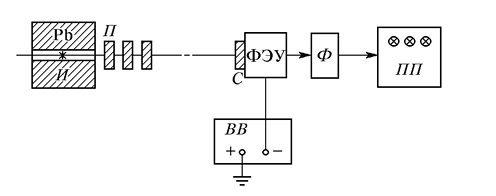
\includegraphics[width=0.5\linewidth]{p1.png}
	\caption{Блок-схема установки, используемой для измерения коэффициентов ослабления потока $\gamma$-лучей: И --- источник $\gamma$-лучей; Pb --- свинцовый контейнер с коллиматорным каналом; П --- набор поглотителей; С --- сцинтиллятор --- кристалл NaI(Tl); Ф --- формирователь-выпрямитель}
	\label{pic_2}
\end{figure}

\begin{figure}[!hb]
	\centering
	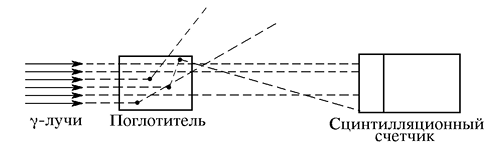
\includegraphics[width=0.5\linewidth]{p2.png}
	\caption{Схема рассеяния $\gamma$ - квантов в поглотителе}
	\label{pic_2}
\end{figure}

\section{Ход работы}

\textbf{1.} Включили пересчетный прибор и высоковольтный выпрямитель и дали им прогреться в течение 10 минут. \par
\textbf{2.} Убедились, что установка чувствует гамма - лучи.\par
\textbf{3.} Исследуем поглощение $\gamma$ - лучей в свинце, железе, алюминии и пробке. 
Для этого измерим число частиц, попадающих на счетчик за фиксированное время в отсутствие $N_{0}$ и в присутствии N поглотителя:\par
$\textbf{В отсутствие поглотителя:}$ $N_{0}$ = 109402 \par

Измерим фон с помощью свинцовой пробки: $N_{\text{фон}}$ = 272 \par

Рассчитаем коэффициенты $\mu '$ по формуле:

\[ \mu ' = \frac{\mu}{\rho}\]

Для Fe: $\mu ' = 0.068 \pm 0.003 $ $\frac{\text{см}^{2}}{\text{г}}$\par
Для Al: $\mu ' = 0.071 \pm 0.003 $ $\frac{\text{см}^{2}}{\text{г}}$\par
Для Pb: $\mu ' = 0.099 \pm 0.003 $ $\frac{\text{см}^{2}}{\text{г}}$\par
Для пробки: $\mu ' = 0.006 \pm 0.001 $ $\frac{\text{см}^{2}}{\text{г}}$\par



\newpage




\begin{table}[h]
\centering
\caption{Серия 1}
\begin{tabular}{|c|c|c|c|c|c|}
\hline
Число брусков & Частицы с фоном & Частицы за 10 сек без фона & $\ln(N_0/N_i)$ & Толщина бруска & $\mu$ \\
\hline
N\_0 & 109402 & 109130 & 0,00 $\pm 0,01$ & 0 $\pm 0,01$& 0,00 $\pm 0,01$ \\
N1 & 60913 & 60641 & 0,59 & 1,03 $\pm 0,01$& 0,57 $\pm 0,01$\\
N2 & 34003 & 33731 & 1,17 & 2,06$\pm 0,03$ & 0,57 $\pm 0,01$\\
N3 & 19822 & 19550 & 1,72 & 3,09$\pm 0,02$& 0,56 $\pm 0,01$\\
N4 & 11662 & 11390 & 2,26 & 4,11$\pm 0,03$ & 0,55 $\pm 0,02$ \\
N5 & 6888 & 6616 & 2,80 & 5,14 $\pm 0,03$& 0,55 $\pm 0,02$ \\
N6 & 3985 & 3713 & 3,38 & 6,17$\pm 0,04$ & 0,55 $\pm 0,02$ \\
N7 & 2537 & 2265 & 3,87 & 7,2 $\pm 0,04$& 0,54 $\pm 0,02$\\
\hline
\end{tabular}
\end{table}

\begin{table}[h]
\centering
\caption{Серия 2}
\begin{tabular}{|c|c|c|c|c|c|}
\hline
Число брусков & Частицы с фоном & Частицы за 10 сек без фона & $\ln(N_0/N_i)$ & Толщина бруска & $\mu$ \\
\hline
N\_0 & 109402 & 109130 & 0,00 & 0  $\pm 0,01$ & 0 $\pm 0,01$ \\
N1 & 72174 & 71902 & 0,42 & 2,1  $\pm 0,02$& 0,20  $\pm 0,01$\\
N2 & 48023 & 47751 & 0,83 & 4,2 $\pm 0,01$ & 0,20  $\pm 0,01$\\
N3 & 32022 & 31750 & 1,23 & 6,3 $\pm 0,02$ & 0,20  $\pm 0,01$\\
N4 & 21864 & 21592 & 1,62 & 8,4 $\pm 0,03$ & 0,19 $\pm 0,02$ \\
N5 & 14706 & 14434 & 2,02 & 10,5 $\pm 0,03$ & 0,19  $\pm 0,02$\\
N6 & 10021 & 9749 & 2,42 & 12,6 $\pm 0,04$ & 0,19 $\pm 0,02$ \\
N7 & 6872 & 6600 & 2,81 & 14,7  $\pm 0,04$& 0,19  $\pm 0,02$\\
\hline
\end{tabular}
\end{table}

\begin{table}[h]
\centering
\caption{Pb}
\begin{tabular}{|c|c|c|c|c|c|}
\hline
Число брусков & Частицы с фоном & Частицы за 10 сек без фона & $\ln(N_0/N_i)$ & Толщина бруска & $\mu$ \\
\hline
N\_0 & 109402 & 109130 & 0,00 & 0 $\pm 0,01$& 0 $\pm 0,02$ \\
N1 & 61219 & 60947 & 0,58 & 0,48 $\pm 0,02$ & 1,21 $\pm 0,02$ \\
N2 & 35538 & 35266 & 1,13 & 0,96 $\pm 0,01$ & 1,18 $\pm 0,01$\\
N3 & 20454 & 20182 & 1,69 & 1,44 $\pm 0,03$ & 1,17 $\pm 0,03$\\
N4 & 12258 & 11986 & 2,21 & 1,92 $\pm 0,04$& 1,15 $\pm 0,03$\\
N5 & 6995 & 6723 & 2,79 & 2,4 $\pm 0,05$& 1,16 $\pm 0,04$\\
N6 & 4301 & 4029 & 3,30 & 2,88 $\pm 0,06$& 1,15 $\pm 0,04$\\
N7 & 2824 & 2552 & 3,76 & 3,36 $\pm 0,06$& 1,12 $\pm 0,04$\\
\hline
\end{tabular}
\end{table}

\begin{table}[h]
\centering
\caption{Пробка}
\begin{tabular}{|c|c|c|c|c|c|}
\hline
Число брусков & Частицы с фоном & Частицы за 10 сек без фона & $\ln(N_0/N_i)$ & Толщина бруска & $\mu$ \\
\hline
N\_0 & 109402 & 109130 & 0,00 & 0,00 $\pm 0,01$ & 0 $\pm 0,001$ \\
N1 & 108188 & 107916 & 0,01 & 1,94 $\pm 0,01$ & 0,006 $\pm 0,001$\\
N2 & 106608 & 106336 & 0,03 & 3,88 $\pm 0,02$ & 0,007 $\pm 0,001$\\
N3 & 103442 & 103170 & 0,06 & 5,82 $\pm 0,03$ & 0,010 $\pm 0,001$\\
N4 & 102422 & 102150 & 0,07 & 7,76 $\pm 0,04$ & 0,009$\pm 0,001$ \\
N5 & 100436 & 100164 & 0,09 & 9,7 $\pm 0,05$ & 0,009 $\pm 0,001$\\
N6 & 98318 & 98046 & 0,11 & 11,64 $\pm 0,06$ & 0,009 $\pm 0,001$\\
N7 & 97237 & 96965 & 0,12 & 13,58 $\pm 0,06$ & 0,009 $\pm 0,001$\\
\hline
\end{tabular}
\end{table}

\newpage

\begin{figure}[!hb]
	\centering
	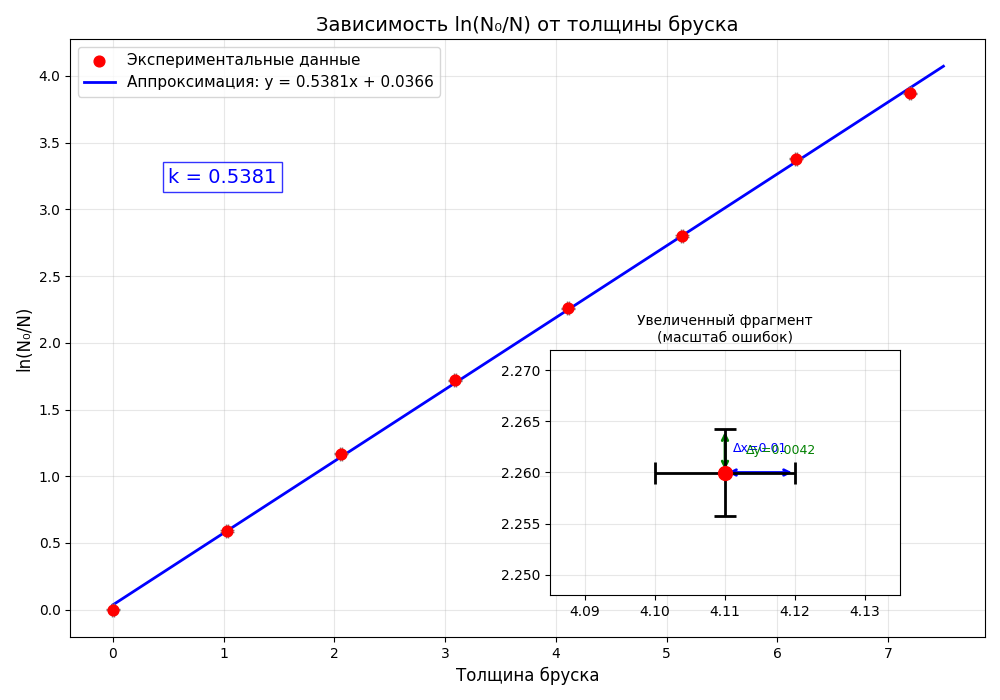
\includegraphics[width=0.5\linewidth]{F1.png}
	\caption{Для Fe}
	\label{pic_2}
\end{figure}


\begin{figure}[!hb]
	\centering
	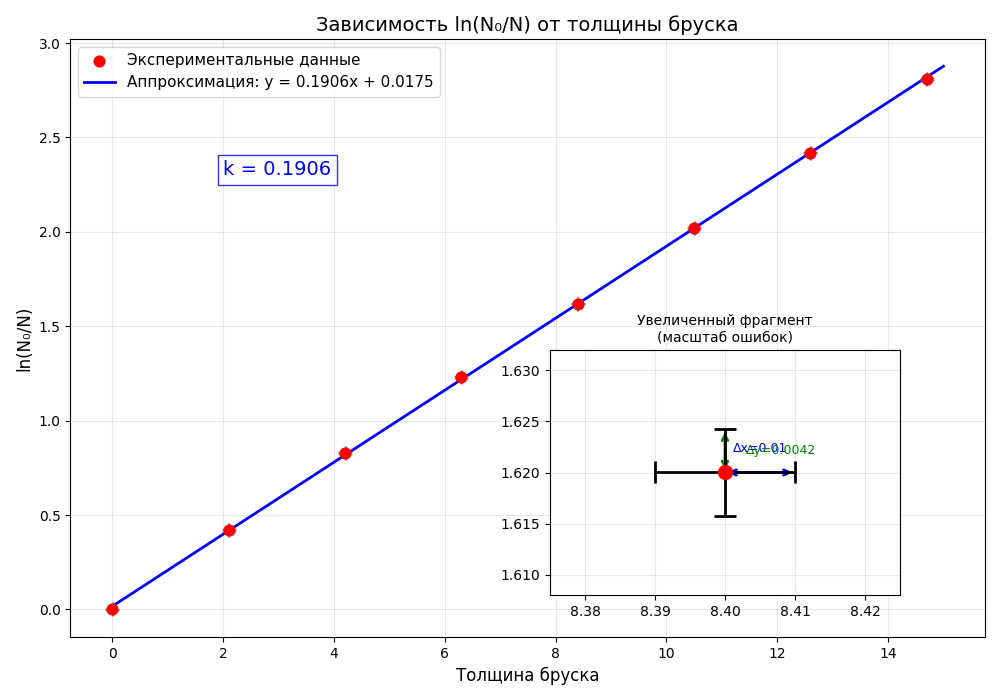
\includegraphics[width=0.5\linewidth]{F2.png}
	\caption{Для Al}
	\label{pic_2}
\end{figure}

\begin{figure}[!hb]
	\centering
	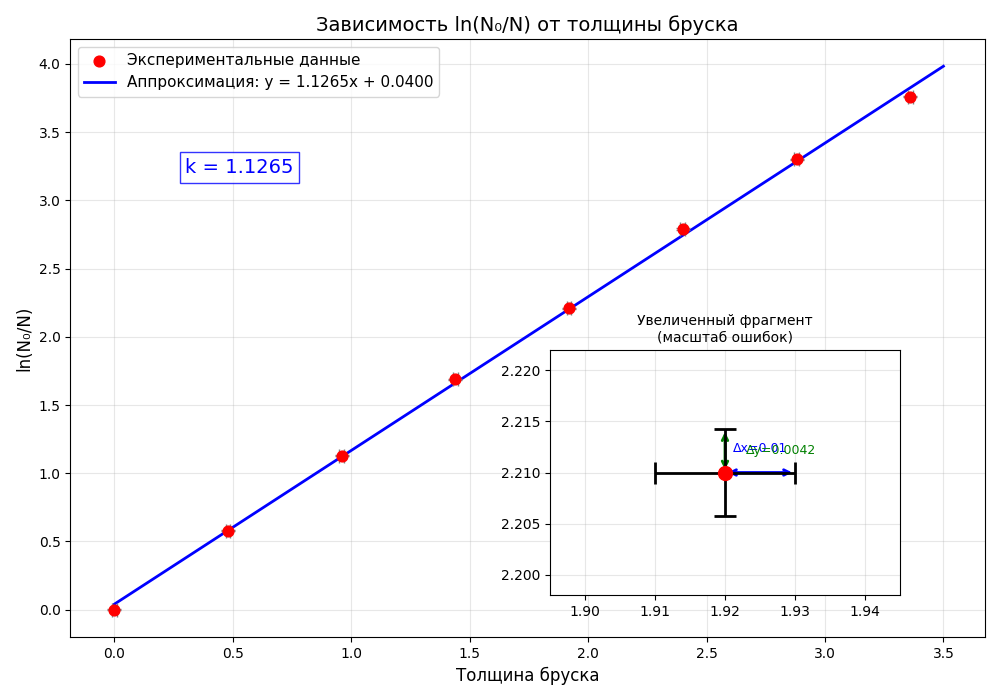
\includegraphics[width=0.5\linewidth]{F3.png}
	\caption{Для Pb}
	\label{pic_2}
\end{figure}

\begin{figure}[!hb]
	\centering
	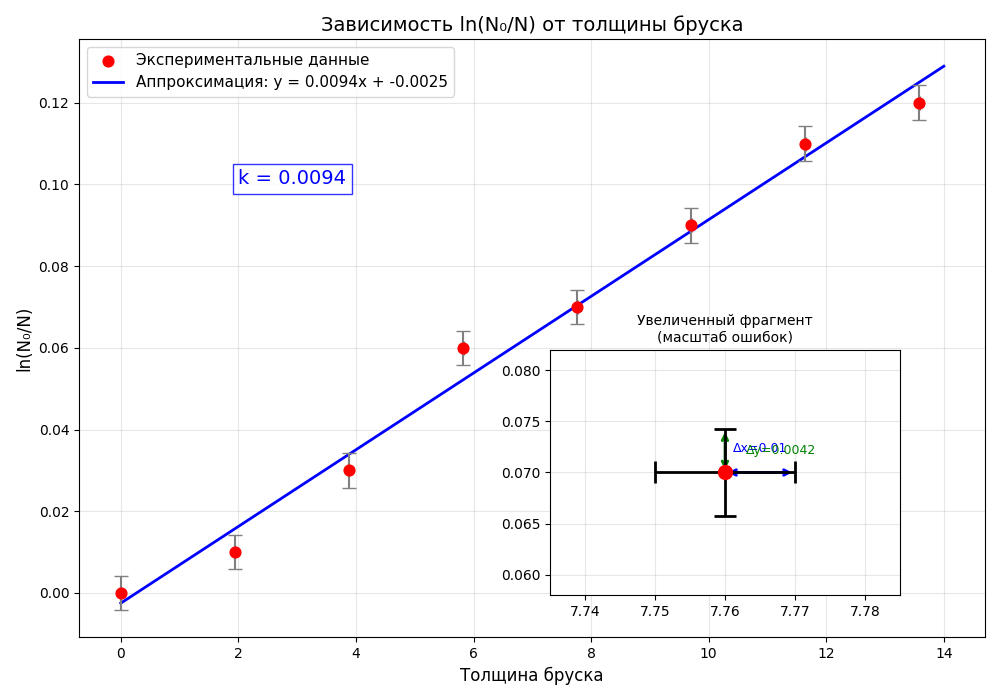
\includegraphics[width=0.5\linewidth]{F4.png}
	\caption{Для пробки}
	\label{pic_2}
\end{figure}

\begin{figure}[!hb]
	\centering
	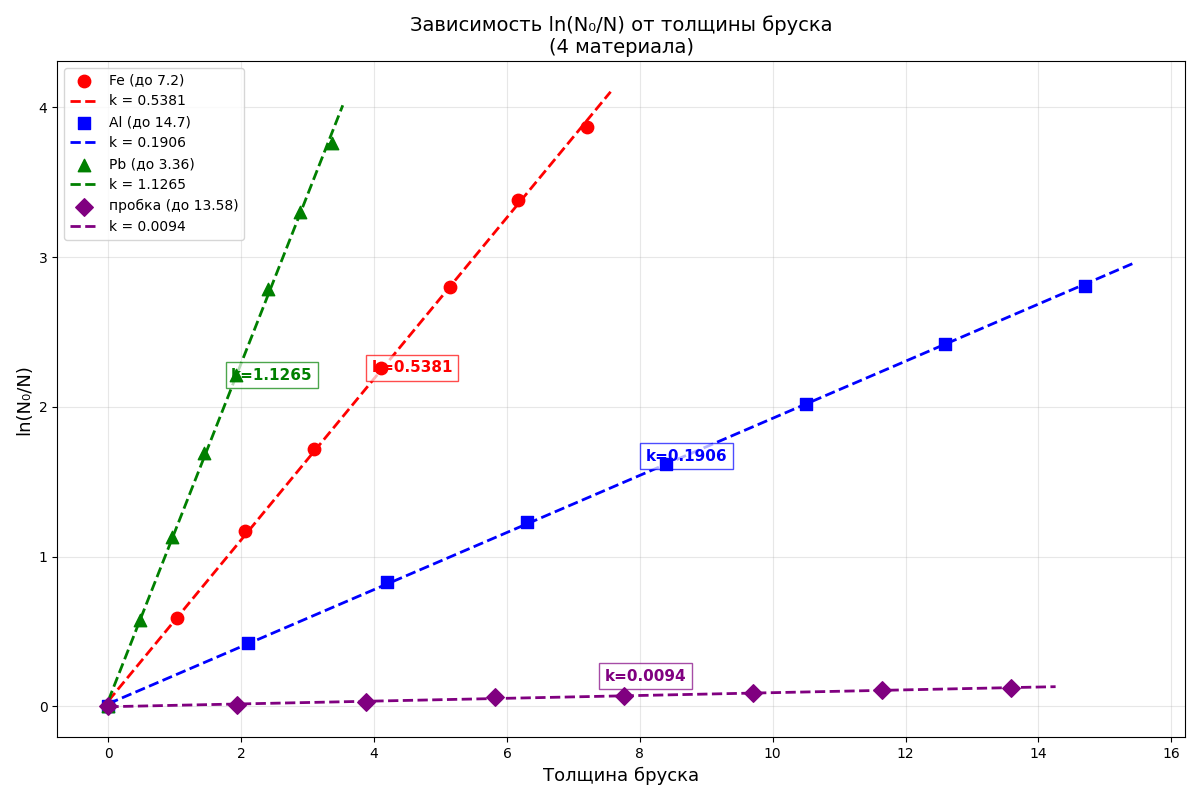
\includegraphics[width=0.5\linewidth]{F5.png}
	\caption{Объединение}
	\label{pic_2}
\end{figure}


% Рассчитаем коэффициенты $\mu '$ по формуле:

% \[ \mu ' = \frac{\mu}{\rho}\]

% Для Fe: $\mu ' = 0.068 \pm 0.003 $ $\frac{\text{см}^{2}}{\text{г}}$\par
% Для Al: $\mu ' = 0.071 \pm 0.003 $ $\frac{\text{см}^{2}}{\text{г}}$\par
% Для Pb: $\mu ' = 0.099 \pm 0.003 $ $\frac{\text{см}^{2}}{\text{г}}$\par
% Для пробки: $\mu ' = 0.006 \pm 0.001 $ $\frac{\text{см}^{2}}{\text{г}}$\par

\newpage

\section{Вывод}

Определил поглощение гамма лучей, рассчитал коэффициенты $\mu$ и $\mu '$, результат оказался близким к табличным данным. По данным коэффициентам ослабления определили по графику среднюю энергию гамма лучей:
по всем материалам это примерно 0,6 МэВ, что соответствует параметрам установки.

\end{document}